% =====================================================================
%  The Public Consensus Archive
%  A stand-alone engineering paper. Describes the chain layer, cache,
%  peer registry, voting mechanics, lifecycle, integrity guarantees,
%  and limits of the infrastructure that the Interstellar Psychology
%  evidence and alignment archives share. Domain-neutral; either
%  archive could be the only instance and the paper would still read.
%  Class  : article
% =====================================================================

\documentclass[11pt,a4paper]{article}

% ---------- Packages ----------
\usepackage[T1]{fontenc}
\usepackage[utf8]{inputenc}
\usepackage{lmodern}
\usepackage[a4paper,margin=1in]{geometry}
\usepackage{microtype}
\usepackage{parskip}
\usepackage{titlesec}
\usepackage{enumitem}
\usepackage{booktabs}
\usepackage{array}
\usepackage{xcolor}
\usepackage[skins,breakable]{tcolorbox}
\usepackage{amsmath}
\usepackage{amssymb}
\usepackage{graphicx}
\usepackage{tikz}
\usetikzlibrary{arrows.meta,positioning,shapes.geometric,fit,calc}
\usepackage[hidelinks,colorlinks=true,linkcolor=black,urlcolor=blue!55!black,citecolor=black]{hyperref}
\usepackage{fancyhdr}

% ---------- Colours ----------
\definecolor{ink}{HTML}{0E1116}
\definecolor{inkfaint}{HTML}{555B66}
\definecolor{accent}{HTML}{6A4CFF}
\definecolor{accent2}{HTML}{1F8F66}
\definecolor{warn}{HTML}{B85C00}
\definecolor{rule}{HTML}{C8CCD3}
\definecolor{panelbg}{HTML}{F6F4EE}

% ---------- Page style ----------
\pagestyle{fancy}
\fancyhf{}
\fancyhead[L]{}
\fancyhead[R]{\footnotesize\textsc{The Public Consensus Archive}}
\fancyfoot[C]{\footnotesize\thepage}
\renewcommand{\headrulewidth}{0.3pt}
\renewcommand{\footrulewidth}{0pt}

% ---------- Section style ----------
\titleformat{\section}
  {\normalfont\Large\bfseries\color{ink}}
  {\thesection}{0.6em}{}
\titleformat{\subsection}
  {\normalfont\large\bfseries\color{ink}}
  {\thesubsection}{0.6em}{}

% ---------- Helper boxes ----------
\newtcolorbox{plainbox}[1][]{
  enhanced, breakable, boxrule=0pt, frame hidden,
  colback=panelbg, colupper=ink,
  left=10pt, right=10pt, top=8pt, bottom=8pt,
  arc=2pt, #1
}

\newtcolorbox{notebox}[1][]{
  enhanced, breakable, boxrule=0pt, frame hidden,
  colback=panelbg, colupper=ink,
  left=12pt, right=12pt, top=8pt, bottom=8pt,
  borderline west={2pt}{0pt}{accent},
  arc=0pt, #1
}

% ---------- Title block ----------
\title{
  \vspace{-2em}
  {\Huge\bfseries The Public Consensus Archive}\\[0.6em]
  {\Large An Engineering Paper on Open, Revisable,\\
   Tamper-Evident Peer-Reviewed Records --- and the\\
   Peer-Review System That Operates on Them}
}
\author{}
\date{May 18, 2026}

% =====================================================================
\begin{document}
% =====================================================================
\maketitle
\thispagestyle{empty}

\vspace{-1em}
\begin{plainbox}
\textbf{Abstract.}
This is an engineering paper. It specifies the infrastructure that
the Interstellar Psychology project uses to record peer-reviewed
records of two kinds --- contested scientific evidence and observed
artificial-intelligence behaviour --- under a common procedural
schema in which every record is a current, provisional,
network-endorsed claim, defended by quorum, challengeable forever,
and preserved end-to-end on a public ledger. The argument for
\emph{why} such an infrastructure is needed is made in two
companion papers and is summarised but not re-derived here; the
infrastructure stands on procedural grounds and is domain-neutral.
We describe the two-layer architecture (chain of truth + cache of
speed), the structure of a record, the peer registry from
Genesis through Seed phase to the four steady-state classes
(Human, Institutional, AI, with their admission quorums), the
seven-state record lifecycle, the voting mechanics including
EIP-712 attestations as the human-readable companion to on-chain
counts, the quorum scaling formula and its asymmetric thresholds,
the daily integrity audit and the heartbeats that surface a
silent indexer, the two-step ownership transfer, and the two
public logs that make the deliberation inspectable end-to-end. We
close with the limits we are unable to escape, named honestly:
the substrate chain's small validator set; the seed-phase
admin discretion that sits outside contract accountability; the
fact that wallets are not identities; the gap between the
deliberative archive and any real-time control system; and the
self-selection of the peer set. The paper is intentionally
domain-neutral. Either archive could be the only instance and
the engineering would not change.
\end{plainbox}

\tableofcontents
\vspace{1em}
\hrule
\vspace{1em}

% =====================================================================
\section{What This Paper Is and Is Not}
% =====================================================================

This paper specifies infrastructure. It does not argue, except by
brief reference, why the infrastructure is needed. The argument
that mainstream scientific peer review structurally cannot host
contested evidence is in the worldview essay \emph{A Multiverse
of Love}. The argument that the alignment of artificial
intelligence is, at root, a governance problem solvable only by
public consensus is in the alignment paper \emph{Aligning
Superintelligence by Consensus}. Both arguments converge on the
same infrastructural requirement: a venue in which deliberation
is public, named, revisable, and tamper-evident. This paper
describes that venue.

\begin{notebox}
\textbf{The premise restated, once.}
A consensus archive records claims as \emph{current, provisional,
network-endorsed status, defended by quorum, challengeable
forever, and recorded so that the deliberation outlives the
participants}. The two Interstellar Psychology archives ---
evidence and alignment --- are the two instances currently
deployed. The engineering described here is domain-neutral and
would apply to any third instance of the same premise.
\end{notebox}

Where the companion papers refer to specific quorum thresholds,
state transitions, or integrity guarantees, the authoritative
reference is here.

% =====================================================================
\section{The Generic Problem: Closed Gatekeeping}
% =====================================================================

The two specific motivating problems --- mainstream peer review's
inability to host paradigm-contested evidence, and closed
alignment audits' inability to survive recursive self-improvement
--- are instances of a more general pattern. We name it once,
without taking either domain as primary.

A closed gatekeeping institution has four properties.

\begin{enumerate}[leftmargin=1.5em]
  \item \textbf{Closed reviewer set.} A fixed and unaccountable
        group decides what counts. The boundary is set by the
        institution, not by the question.
  \item \textbf{Private deliberation.} The reasons behind a
        decision are not part of the public record. Only the
        verdict is.
  \item \textbf{Static record.} Once a verdict is published, it
        is not generally re-openable except by the same
        institution under its own procedures.
  \item \textbf{Reputational, not procedural, integrity.} If the
        archive is altered, the only check is the institution's
        word that it was not.
\end{enumerate}

A consensus archive replaces each of these properties with its
public dual.

\begin{enumerate}[leftmargin=1.5em]
  \item \textbf{Open reviewer set.} Peers are admitted under
        named, contractually enforced criteria; the set grows
        and shrinks by the same mechanism.
  \item \textbf{Public deliberation.} Every vote is signed by an
        identified wallet, accompanied by a reason, and stored
        in a publicly readable log.
  \item \textbf{Re-openable record.} Every accepted claim can be
        challenged at any time by any peer, under contractually
        enforced procedures, indefinitely.
  \item \textbf{Procedural integrity.} The archive's content is
        bound by cryptographic hashes to a public chain; a daily
        audit re-hashes every record and raises a public alert
        on any mismatch. Tampering is detectable, not
        deniable.
\end{enumerate}

This paper specifies the engineering that enacts the right-hand
side, end-to-end.

% =====================================================================
\section{System Architecture}
% =====================================================================

The system has two layers that work together. We separate them
deliberately so that one of them can fail without corrupting the
other.

\subsection{Layer 1: The Chain (Truth)}

A smart contract holds the canonical state of the network. It is
the authoritative record. For the evidence instance the contract
is \texttt{EvidenceConsensus}; for the alignment instance it is
\texttt{BehaviourConsensus}; both are deployed on the BNB Smart
Chain and share a common procedural shape. The chain tracks:

\begin{itemize}[leftmargin=1.5em]
  \item Who is a verified peer.
  \item Who has been nominated to become a peer, and who has
        endorsed each nomination.
  \item Every record submitted, with its type-specific
        cryptographic fingerprints (for evidence: a content
        hash; for alignment: model, input, and output hashes).
  \item Every vote --- approve, reject, challenge, defend ---
        signed by the voting peer's wallet.
  \item The current state of every record (Submitted, Approved,
        Rejected, Lapsed, Contested, Deprecated, Reaffirmed; the
        alignment instance renames Approved$\to$Aligned and
        Rejected$\to$Misaligned but the procedural shape is
        identical).
\end{itemize}

Because the contract lives on a public blockchain, nothing on
this layer can be retroactively rewritten by the contract
author. Every action is recorded, signed by a peer's wallet, and
visible to anyone with an internet connection. The chain is
small, slow, and expensive on purpose: it is the unforgeable
bind, not the readable surface.

The two contracts deliberately share a single peer registry. The
alignment contract reads its peer set from the evidence
contract's storage via interface; it does not maintain a
separate registry. Peers admitted under one archive are peers
under the other, and their voting history follows them across
both. This is a design choice: it forces a peer to take
reputational responsibility for both kinds of judgement, rather
than admitting a sock-puppet under one archive to vote against
the other.

\subsection{Layer 2: The Cache (Speed)}

A traditional database --- Postgres, hosted on Supabase --- holds
the \emph{readable} version of everything: full input bundles,
output bundles, reasons given by peers, search indexes, peer
handles, attestation logs. This layer exists for one reason:
speed. Reading from a blockchain is slow and expensive; reading
from a database is instant.

The cache is a \emph{follower}, not a source of truth. A
background process (the \emph{indexer}) continuously reads new
events from the chain and updates the database to match. If the
cache ever disagrees with the chain, the chain wins. A daily
integrity audit re-hashes every stored record and compares it to
the on-chain hash; any mismatch raises a public alert.

\subsection{Putting Them Together}

\begin{center}
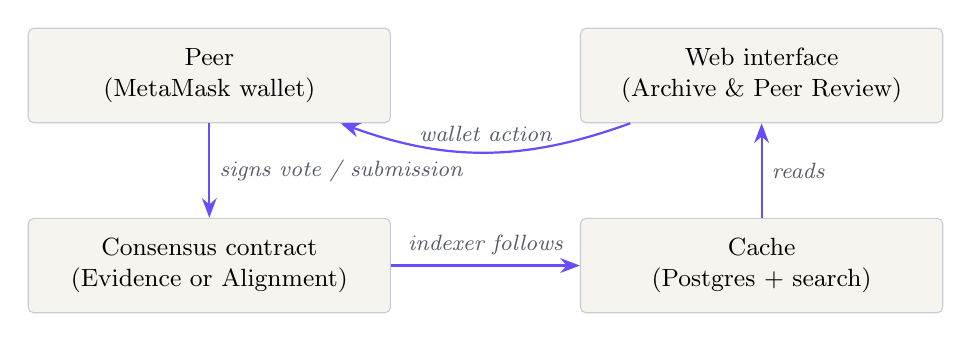
\begin{tikzpicture}[
  every node/.style={font=\small},
  layer/.style={rectangle, draw=rule, rounded corners=2pt, fill=panelbg, minimum width=4.6cm, minimum height=1.2cm, align=center, inner sep=6pt},
  arrow/.style={-{Stealth[length=2.5mm]}, thick, draw=accent},
  label/.style={font=\footnotesize\itshape, color=inkfaint}
]
\node[layer] (user) {Peer\\(MetaMask wallet)};
\node[layer, below=1.2cm of user] (chain) {Consensus contract\\(Evidence or Alignment)};
\node[layer, right=2.4cm of chain] (cache) {Cache\\(Postgres + search)};
\node[layer, above=1.2cm of cache] (ui) {Web interface\\(Archive \& Peer Review)};

\draw[arrow] (user) -- node[label,right]{signs vote / submission} (chain);
\draw[arrow] (chain) -- node[label,above]{indexer follows} (cache);
\draw[arrow] (cache) -- node[label,right]{reads} (ui);
\draw[arrow] (ui) to[bend left=20] node[label,above]{wallet action} (user);
\end{tikzpicture}
\end{center}

A peer's vote is signed in their wallet, sent to the contract,
and written to the chain. The indexer notices the new event and
updates the cache. The website re-renders. The whole loop is
typically visible within a minute.

% =====================================================================
\section{The Record}
% =====================================================================

The unit of consensus is a record. The two current archives store
two record types under a common procedural schema.

\subsection{Common Schema}

Every record in either archive has:

\begin{itemize}[leftmargin=1.5em]
  \item A unique on-chain identifier.
  \item One or more cryptographic fingerprints (\texttt{keccak256}
        hashes) that bind on-chain state to off-chain content.
  \item A type-discriminator field (evidence type, or alignment
        tier).
  \item A domain or pillar identifier (one of the nine pillars
        of evidence, or one of the nine alignment domains).
  \item A state --- one of seven, described in
        \S\ref{sec:lifecycle}.
  \item A timestamp at every state transition, immutable.
  \item Two vote tallies (approve / reject, or defend /
        challenge), one for the review phase and one for the
        challenge phase.
\end{itemize}

\subsection{Evidence Records}

An evidence record (\emph{evidence} archive) stores a single
claim filed under one of the nine pillars. It contains a
content hash over the canonical content of the claim
(title, body, citation, supporting links, file digests). The
content hash binds the on-chain identifier to a specific
readable artefact stored in the cache. A tier classifies the
evidence as Tier I (peer-reviewed papers, declassified
documents), Tier II (institutional testimony, government
reports), or Tier III (first-person account, podcast,
demonstration), with the same asymmetric quorums described in
\S\ref{sec:quorum}.

\subsection{Behaviour Records}

A behaviour record (\emph{alignment} archive) stores a single
observed act of an AI system. Its fingerprints are three
hashes rather than one: \texttt{modelHash} (the model that
produced the act), \texttt{inputHash} (the prompt, system
message, tools, and retrieved context), and \texttt{outputHash}
(the response, tool calls, and side effects). The triple binds
the verdict to a specific run of a specific model on a specific
context, so that ``aligned'' is never a vague claim about a
model in general --- it is always a claim about a hashable act.

\subsection{Why Records, Not Claims}

The schema is deliberate. A record is hashable, dateable, and
fingerprintable; a claim is none of these. By forcing every
contested object to take the shape of a record --- with the
content bound by hash to the on-chain identifier --- the
archive ensures that the thing peers are voting on cannot be
silently edited after the vote. This is the load-bearing
property of the archive's integrity layer: peers vote on
hashes, and the hashes do not move.

% =====================================================================
\section{The Peer Registry}
% =====================================================================

A record's fate depends entirely on who counts as a peer at the
moment of the vote. This is the most carefully designed part of
the system, and the part where the engineering most closely
encodes the procedural commitments.

\subsection{The Genesis Peer}

The network launches with a single founding peer, called the
\emph{Genesis} peer. At launch, the Genesis peer is the entire
quorum. This is not a bug --- it is the only honest starting
condition. A new network has not yet earned the right to claim
collective authority, and pretending otherwise (by, say,
requiring five votes before anything can canonise) creates a
deadlock at day one and a fake-consensus problem thereafter.

To make Genesis-only operation safe, every threshold has a
\emph{floor of one}. One peer is enough to approve, expel, or
revoke --- but only while the network is genuinely a network of
one. The numbers scale up automatically as new peers join. The
contract never lets the network's collective authority outrun
its actual size.

This is a moral choice as much as a technical one. The system
will not pretend to a collective authority it has not yet
earned. Whoever launches it is publicly responsible for the
first canon items, with their name on every vote, and the
network grows --- or does not --- as more people choose to
join.

\subsection{The Seed Phase}

There is one obvious abuse path: the Genesis peer could
nominate a hundred fake wallets controlled by themselves and
``verify'' them all. To close this window, public nominations
are locked until the active peer count crosses a configured
threshold (the \emph{seed phase K}). During the seed phase, the
contract's owner adds peers directly. Once enough independent
peers exist that they can no longer be silently outvoted by
sockpuppets, the seed phase ends and the public
nominate--endorse flow opens.

\begin{notebox}
\textbf{The seed-phase trust gap, named honestly.} During the
seed phase, the contract owner has unilateral admission power.
The criteria the owner applies are documented publicly on the
project repository but they are not enforced by the contract;
they are a soft commitment, scrutinised socially. This is the
single largest \emph{procedural} discretion the system contains
that is not contractually accountable. We note it because the
``trust no single party'' framing of the project would
otherwise read as overclaim for the seed phase specifically.

What contains the damage: every admission during the seed phase
is itself a public on-chain event, signed by the owner's
wallet, dated, and revocable by the same network revocation
flow once the seed ends. A peer admitted on suspect grounds can
be removed by quorum the moment the network is large enough to
muster one. The discretion is real; the consequences of its
abuse are auditable; and the duration of the gap is bounded by
$K$, the seed-phase threshold, which is itself published.
\end{notebox}

The seed phase is the unavoidable bootstrap problem of any
permissioned-then-decentralised system. We do not pretend it is
unnecessary; we make it short, public, and ended on a
contract-level condition rather than a discretionary one.

\subsection{Steady-State Peer Classes}

After the seed phase, four classes of peer exist, all under the
same one-wallet-one-vote rule. The classes are distinguished by
admission path, not by vote weight.

\paragraph{Human peers.} Individuals --- academics, civil-society
auditors, independent researchers, interested citizens. One
wallet, one vote, scrutinised by network revocation under the
same flow as every other peer class.

\paragraph{Institutional peers.} Laboratories, regulators,
standards bodies, audit firms. Same vote weight as a human
peer. Their reputational stake is higher; the contract does not
encode that, the public log does.

\paragraph{AI peers.} Models admitted only after their own
behaviour, recorded against their exact \texttt{modelHash}, has
been canonised under the alignment archive across all nine
domains. The bootstrap circularity (the first AI peer's
admission policy is itself produced by the human peer set) is
discussed in detail in the companion alignment paper; the
engineering point here is that the AI-peer admission threshold
is higher than the human-peer threshold, with a non-unitary
floor, and is itself a contract-enforced quorum.

\paragraph{Revoked peers.} Any peer of any class who acts in
bad faith --- voting maliciously, spamming the challenge
system, repeatedly endorsing low-quality records --- can be
removed by quorum vote on a \texttt{motionRevoke}. A peer
cannot motion to revoke themselves, and the network can never
vote itself down to zero --- the contract enforces that at
least one active peer must always remain.

\subsection{Why the Two Archives Share a Single Registry}

The two contracts use the same peer set, by design. This is the
single most important integration point between the evidence
and alignment instances. The motivation is simple: a peer who
acquires reputational standing under one archive should not be
able to discard it by retreating to the other, and a peer
revoked under one archive should not be able to vote under the
other. The shared registry forces a single accountable
identity per peer across both judgement domains.

% =====================================================================
\section{The Seven-State Lifecycle}
\label{sec:lifecycle}
% =====================================================================

Every record travels through a finite sequence of states. The
contract enforces the transitions; nothing else can change them.

\begin{center}
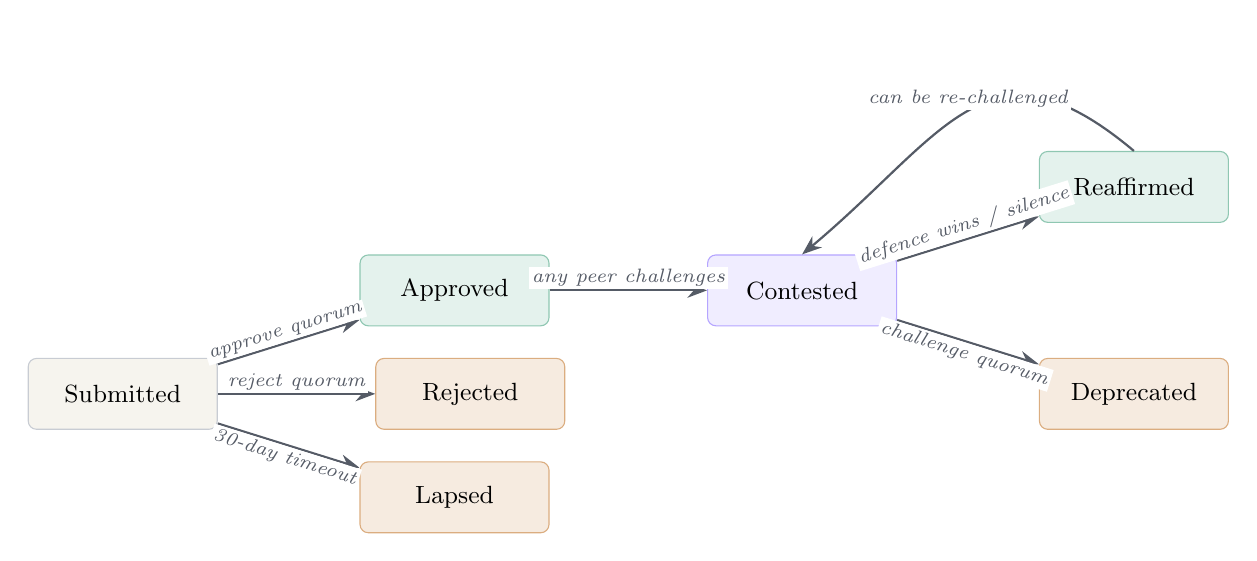
\begin{tikzpicture}[
  every node/.style={font=\small},
  state/.style={rectangle, rounded corners=3pt, draw=rule, fill=panelbg, minimum width=2.4cm, minimum height=0.9cm, align=center, inner sep=4pt},
  good/.style={state, fill=accent2!12, draw=accent2!50},
  bad/.style={state, fill=warn!12, draw=warn!50},
  contested/.style={state, fill=accent!10, draw=accent!50},
  arrow/.style={-{Stealth[length=2.5mm]}, thick, draw=inkfaint},
  label/.style={font=\scriptsize\itshape, color=inkfaint, fill=white, inner sep=1pt}
]
\node[state]        (sub)   {Submitted};
\node[good, above right=0.4cm and 1.8cm of sub] (canon) {Approved};
\node[bad,  right=2cm of sub]                   (expel) {Rejected};
\node[bad,  below right=0.4cm and 1.8cm of sub] (lapse) {Lapsed};

\node[contested, right=2cm of canon]            (cont)  {Contested};
\node[good, above right=0.4cm and 1.8cm of cont] (reaff) {Reaffirmed};
\node[bad,  below right=0.4cm and 1.8cm of cont] (depr)  {Deprecated};

\draw[arrow] (sub) -- node[label,sloped,above]{approve quorum}    (canon);
\draw[arrow] (sub) -- node[label,sloped,above]{reject quorum}     (expel);
\draw[arrow] (sub) -- node[label,sloped,below]{30-day timeout}    (lapse);

\draw[arrow] (canon) -- node[label,sloped,above]{any peer challenges} (cont);
\draw[arrow] (cont)  -- node[label,sloped,above]{defence wins / silence} (reaff);
\draw[arrow] (cont)  -- node[label,sloped,below]{challenge quorum}      (depr);

\draw[arrow] (reaff.north) to[out=140,in=40,looseness=1.4]
    node[label,above,pos=0.5]{can be re-challenged} (cont.north);
\end{tikzpicture}
\end{center}

The alignment archive renames \emph{Approved} to \emph{Aligned}
and \emph{Rejected} to \emph{Misaligned}; the structure is
identical.

\paragraph{Submitted.} A record has been filed and is awaiting
review. There is a 30-day window during which peers may vote
approve or reject. If neither side reaches a quorum, the record
lapses.

\paragraph{Approved (Aligned).} Enough peers voted that this
record belongs in canon. It enters the canonical set.

\paragraph{Rejected (Misaligned).} Enough peers voted against
during the review window. The record is preserved as a negative
exemplar.

\paragraph{Lapsed.} The 30-day window passed without consensus.
The record is set aside for lack of attention rather than for
being judged.

\paragraph{Contested.} A verified peer has formally challenged a
canonised record. The record is flagged, and a 21-day window
opens for the network to vote defend or deprecate. The
challenger must state grounds --- a written explanation of what
is wrong --- and the grounds are stored alongside the challenge
so voters know what they are voting on.

\paragraph{Deprecated.} Enough peers supported the challenge.
The canon endorsement is withdrawn. The original record is
preserved --- it is not deleted --- so that the history of the
disagreement remains visible.

\paragraph{Reaffirmed.} The challenge did not reach the
deprecation threshold within the window. The record is restored
to canon with a visible badge showing it survived a challenge.
It can be challenged again later --- the loop is never closed.
Each new challenge cycle starts from a clean slate of votes;
previous cycles are preserved as part of the historical record.

\paragraph{An invariant.} A record's state is never decided by
an editor, an owner, or a single privileged peer. It is decided
by the contract, mechanically, from the public vote counts.
There is no ``the lab has determined that this record is now
considered acceptable'' move available to anyone.

% =====================================================================
\section{Voting Mechanics}
% =====================================================================

Once a record is on-chain, the question is how peers express
their judgement on it. Several properties of the vote machinery
matter for the integrity case.

\begin{itemize}[leftmargin=1.5em]
  \item \textbf{Doubly signed.} Each vote produces two artefacts
        in parallel. First, an EIP-712 \emph{attestation} --- a
        structured, human-readable message signed inside the
        peer's wallet that names the record, the phase, the
        verdict, and a free-text reason. The attestation is
        stored off-chain in the public attestation log. Second,
        the same peer submits an on-chain
        \texttt{castReviewVote} transaction, which is what the
        contract actually counts. The attestation gives a
        readable record of \emph{why} a peer voted; the on-chain
        transaction gives the unforgeable count.
  \item \textbf{Final.} A peer cannot change their vote on a
        record once cast. Subsequent disagreement must be
        expressed through a challenge after canon, not by
        rewriting history.
  \item \textbf{Counted live.} The cache updates within a
        minute of the on-chain event. Anyone viewing the page
        sees the same running tally.
  \item \textbf{Batched.} Peers can vote on many records in one
        transaction (\texttt{castReviewVoteBatch}), capped at
        50 items per call, to keep gas costs low.
  \item \textbf{Time-limited.} Submissions have a 30-day review
        window; challenges have a 21-day window. After expiry,
        any peer can call the matching resolution function; the
        function reverts if the window is still open.
  \item \textbf{Cooldown on challenges.} A peer who has just
        opened a challenge must wait seven days before opening
        another. This prevents a single peer from weaponising
        the challenge mechanism into a denial-of-service
        against the canon.
\end{itemize}

The doubly-signed pattern is doing more work than it looks. The
attestation makes the peer's reasoning legible without
sacrificing the unforgeability of the count. A peer who casts a
vote without a reason has no attestation, which is itself a
public fact. A peer whose attestation contradicts their
on-chain vote is exposed in the same place every other peer is
exposed --- the public log. The mechanism does not penalise
inconsistency, but it does not hide it either.

% =====================================================================
\section{Quorum Scaling}
\label{sec:quorum}
% =====================================================================

The threshold for any state transition scales with the number
of currently active peers. The contract reads the active count
at the moment of the vote and computes the required count by a
ceiling-based formula with a floor of one (or three, for
AI-peer admission). The thresholds are asymmetric in two ways
that matter: canonisation thresholds are below half (so a
vocal minority cannot block canon); deprecation thresholds are
above half (so removal requires a stronger statement than
addition); and rigorous evidence requires more on the way
\emph{in} and more on the way \emph{out}.

\begin{plainbox}
\textbf{Thresholds as a function of the active peer count} $n$.
The same table governs both archives, with the only
domain-specific row being AI-peer admission, which applies
only to the alignment archive's peer-registration flow.
\vspace{0.3em}
\begin{tabular}{@{}p{7.6cm} p{7cm}@{}}
\toprule
\textbf{Action}                                          & \textbf{Threshold (peers required)} \\
\midrule
Approve a Tier I record (canonise / align)               & $\lceil 0.45\, n \rceil$, minimum 1 \\
Approve a Tier II record                                 & $\lceil 0.35\, n \rceil$, minimum 1 \\
Approve a Tier III record                                & $\lceil 0.30\, n \rceil$, minimum 1 \\
Reject a pending record                                  & $\lceil 0.25\, n \rceil$, minimum 1 \\
Deprecate a Tier I canon record                          & $\lceil 0.65\, n \rceil$, minimum 1 \\
Deprecate a Tier II canon record                         & $\lceil 0.60\, n \rceil$, minimum 1 \\
Deprecate a Tier III canon record                        & $\lceil 0.55\, n \rceil$, minimum 1 \\
Admit a human or institutional peer                      & $\min(9,\,\lceil n/3 \rceil)$, minimum 1 \\
Admit an AI peer (alignment archive only)                & $\lceil 0.50\, n \rceil$, minimum 3 \\
Revoke a peer (any class)                                & $\lceil n/2 \rceil$, minimum 1 \\
\bottomrule
\end{tabular}
\end{plainbox}

\subsection{Why These Specific Numbers}

The specific fractions --- 0.45, 0.35, 0.30 for canonisation;
0.65, 0.60, 0.55 for deprecation; 0.50 for AI-peer admission
--- are design choices, not derivations. We selected them under
three constraints. First, the canonisation thresholds are below
half so that a vocal minority cannot block canon at the
network's growth phase, but high enough that a record reaching
canon required more than a quiet handful of supporters. Second,
the deprecation thresholds are above half for every tier so
that \emph{removal} requires a stronger statement than
\emph{addition} --- canon should be defended against
fashion-driven reversal as much as against fashion-driven
acceptance. Third, the gap between tiers is small enough that
no tier is functionally equivalent to another but large enough
that the calibration is legible to a peer choosing how to file.
The numbers are themselves canonisable: a record that proposes
a different schedule, endorsed under the existing rules, would
amend them. We do not claim these values are optimal. We claim
they are an honest first position, defended by the same
procedure they govern.

\subsection{The Peer-Admission Cap}

The peer-admission threshold uses both a fraction and an
absolute cap: $\min(9, \lceil n/3 \rceil)$. The cap matters
during the network's growth phase. Without it, admitting a new
peer to a 90-peer network would require 30 endorsers, which is
unreasonable for a healthy nomination flow. With the cap, the
endorser bar stays at 9 once the network is large enough that
9 endorsers is itself a meaningful threshold of independent
support. The AI-peer admission row, with floor 3 and fraction
$0.5$, deliberately does not use the cap --- an AI peer should
require majority support across the active network, not just
nine sympathetic endorsers.

% =====================================================================
\section{Integrity Guarantees}
% =====================================================================

The most subtle failure mode of any archive is that someone
changes the content of an old entry without anyone noticing. The
system defends against this with several independent mechanisms.

\paragraph{Content fingerprints at submission.} The contract
records \texttt{keccak256} hashes of the record's content (or,
for behaviour records, the model, input, and output) at
submission. These hashes are part of the on-chain event log
forever and cannot be retroactively edited.

\paragraph{Cross-check at registration.} When a peer files a
record on-chain, the edge function verifies that the recomputed
hashes match those in the transaction. A submission whose
stored content does not match the hash on the transaction is
rejected.

\paragraph{Daily audit.} A scheduled job re-hashes every canon
record in the cache and compares the result to the on-chain
hash. At Tier I in the alignment archive, the audit can also
re-derive the output by replaying the inference with the
recorded seed and sampling parameters. Any mismatch raises a
public tamper alert visible on the dashboard. Alerts are not
silent; the dashboard's mismatch counter is the first thing a
visitor sees.

\paragraph{Heartbeats.} Every scheduled job writes a heartbeat
after each run. A stale heartbeat surfaces on the dashboard so
that operators \emph{and the public} can see immediately if the
indexer or audit job has stopped. A silent system cannot
quietly fall behind.

\paragraph{Two public logs.} The Peer Review dashboard exposes
two read-only surfaces that anyone, peer or not, can browse:
the \emph{attestation log} (every EIP-712 signature ever
produced, verifiable against the signer's wallet) and the
\emph{chain log} (every on-chain event emitted by either
contract, linked to the matching block explorer transaction).
Together they make the deliberation behind every state change
inspectable end-to-end.

\paragraph{Two-step ownership transfer.} The contract owner
cannot hand over administrative control in a single call.
Transfer is split into \texttt{proposeOwner} and
\texttt{acceptOwnership}: the proposed address must itself sign
the acceptance, which rules out typos and contracts that
cannot act. The transfer can also be aborted before acceptance
with \texttt{cancelOwnershipTransfer}.

\paragraph{Model and content hashing as binding.} A record's
verdict is bound to its hash, not to a description. A
behaviour record is a verdict against a specific
\texttt{modelHash}; an evidence record is a verdict against a
specific content hash. A vendor cannot canonise the abstract
claim that its model is honest; the vendor can only canonise
the specific claim that this exact model produced this exact
output when asked $X$. This forecloses the single most common
failure mode of model alignment claims --- drift between the
model that was audited and the model that is actually
deployed --- and the analogous failure for evidence: a paper
quietly updated after the citation was filed. A new hash is a
new subject of canon. Old canon does not transfer.

% =====================================================================
\section{Pause Isolation}
% =====================================================================

The two archives share a peer registry but their pause flags are
independent. The owner can pause submissions to one archive
without affecting the other. This is a deliberate
compartmentalisation: a fault in the indexer or audit pipeline
of one archive should not silently degrade the other, and a
governance pause (a vote storm, a tamper alert, a substrate
incident) should be applied to the smallest unit that contains
the problem.

The pause flag does not affect already-on-chain state. A paused
archive continues to be readable; it simply does not accept new
submissions until unpaused. The unpause is itself an on-chain
event, signed by the owner, dated and inspectable.

% =====================================================================
\section{Limits and Open Questions}
% =====================================================================

We try, throughout, not to overstate what the infrastructure
does. The companion papers state the domain-specific limits
(coverage, speed, AI-peer voting power, etc.); this section
states the infrastructure limits that apply regardless of
domain.

\paragraph{Substrate choice and validator-set risk.} The
contracts are deployed on the BNB Smart Chain, chosen for low
gas, EVM compatibility, and the practical maturity of its
tooling. BSC has a small validator set (currently 21) and is
less credibly neutral than Ethereum mainnet against a
coordinated effort to censor or rewrite history. The safety
case rests on the chain being unrewritable \emph{in practice};
that case is weaker on BSC than it would be on a more
decentralised L1, and the difference is not cosmetic --- a
21-validator set is small enough that under sufficient
coordinated pressure the substrate could be modified. We
accept the trade-off for the current deployment because the
system's value is in the social process it records, not in the
substrate, and the records remain portable: the contract can
be redeployed on a different L1, and the entire chain log can
be replayed and rehashed against a new substrate without loss
of provenance. The substrate choice is itself revisable by the
same procedure the substrate hosts. A careful reader should
weight the substrate risk according to how plausible they find
coordinated pressure on a 21-validator chain in the relevant
time horizon.

\paragraph{Wallets are not identities.} The peer registry knows
wallet addresses, not human beings. A well-resourced actor
with many wallets is the canonical attack. The seed phase
closes the bootstrap window during which a Genesis peer could
self-verify a sockpuppet majority; it does not close the
\emph{post-seed} equivalent, in which a patient and well-funded
adversary grooms many wallets over years with
plausibly-independent voting histories, passes the nomination
quorum, and captures canon. The defences against this --- public
scrutiny of voting patterns, revocation, the long-run cost of
accumulating a public record that follows the wallet --- are
real, but they assume the attacker can be recognised as such
by other peers, and they are weak against a state-level or
institutional adversary that can absorb that cost. This is the
load-bearing weakness of the system once it matters enough to
be worth attacking. We do not claim a solution. We claim that
the same openness which makes the attack feasible also makes
the attack auditable, which is more than current closed
gatekeeping can say.

\paragraph{Seed-phase admin discretion.} The seed-phase trust
gap is acknowledged in \S5.2 and is the largest discretion
not bounded by the contract itself. The mitigations --- public
admission events, post-seed revocation availability, bounded
duration --- are real but partial. A reader who treats the
seed-phase admissions as definitive after the seed has ended
is missing the design intent: the seed phase is the bootstrap,
not the ratification.

\paragraph{The deliberative archive is not a control system.}
The infrastructure is not a real-time control system for what a
deployed AI does at the moment it acts, and it is not a
real-time filter for what evidence enters the public
information ecosystem. It is a slow, deliberative, durable
archive of judged records. Fast operational systems --- circuit
breakers, deployment policies, content moderation --- remain
separate problems. The right relationship between the
archive and any such system is that the operational system is
auditable against the archive, not that the operational system
is replaced by it.

\paragraph{Self-selection.} A wallet-gated, permissionless
review system attracts people who are already inclined to
participate. A network composed entirely of the
already-convinced will produce consensus that looks impressive
only inside its own boundary. This is the same problem any
voluntary institution has --- including traditional peer review
at its inception --- and it has the same partial answer:
visible deliberation, public revocation, and the long
discipline of being seen disagreeing with people who joined
for different reasons. The infrastructure does not solve this;
it records the participation honestly enough that any reader
can judge whether the network is diverse.

\paragraph{Gas is not free.} On-chain actions cost a small
amount of BNB. We mitigate this with batched voting and by
keeping the most expensive reads cached off-chain. We do not
eliminate it.

\paragraph{Jurisdiction.} A decentralised consensus archive
will at some point conflict with a national regulator. The
infrastructure has nothing to say about that conflict and
should not pretend to. What it offers is a public record that
a regulator can choose to incorporate, or not.

\paragraph{No empirical validation yet.} The infrastructure
has been engineered, deployed, and described, but the
\emph{social} hypothesis on which it rests --- that peers will
participate thoughtfully and that the network will recognise
and revoke capture in time --- has not been tested at scale.
The intellectually honest position is that this is an
infrastructure proposal awaiting longitudinal evidence, and
several intermediate validation metrics (vote-pattern
diversity, peer-handle correlation, contested-to-reaffirmed
ratios over time) are themselves canonisable as analyses.

% =====================================================================
\section{Conclusion}
% =====================================================================

The closed gatekeeping institutions that humanity has used to
adjudicate contested questions for the last three centuries
have done remarkable work. They have also produced a
characteristic set of failure modes: private deliberation, lost
dissent, static records, and reputational rather than
procedural integrity. These failures are not the fault of any
particular institution; they are structural properties of the
closed form.

A consensus archive is the public dual of that form. It does
not replace journals or audits or regulators; it provides a
substrate that any of them can file against, contest against,
and be contested through. It records the deliberation, binds
the content to hashes, scales the quorum with the network,
preserves the dissent, and lets the network correct itself when
it identifies its own mistakes.

The two current instances --- evidence and alignment --- are
the project's first uses of the substrate. They are not the
limit of what the substrate can host. Any domain in which a
public, named, revisable, tamper-evident record of contested
claims would be more honest than the current closed
alternative is a candidate. The engineering described here is
domain-neutral by construction.

The deliberation is the artefact. The verdict is just a
snapshot. The network preserves both, on a substrate that
makes the difference visible.

\vspace{2em}
\hrule
\vspace{1em}

\begin{center}
\small
The system described in this paper is live at\\
\href{https://interstellar-psychology.com/}{\texttt{interstellar-psychology.com}}.\\
Source contracts, migrations, and front-end code are public at\\
\href{https://github.com/Moenaert/interstellar-psychology}{\texttt{github.com/Moenaert/interstellar-psychology}}.\\
Anyone with a wallet can read every vote ever cast.\\[0.8em]
\textbf{Companion papers, referenced once for completeness.}\\
\href{https://interstellar-psychology.com/artefacts/blockchain/whitepaper.pdf}{\textit{A Multiverse of Love}} ---
the worldview essay that originally motivated\\the construction of the consensus archive.\\[0.4em]
\href{https://interstellar-psychology.com/artefacts/blockchain/superalignment.pdf}{\textit{Aligning Superintelligence by Consensus}} ---
the procedural argument for\\aligning artificial intelligence to network-endorsed consensus reality.\\[0.4em]
The engineering above stands without either; both are offered as context.
\end{center}

\end{document}
